Dans l'ensemble des travaux entrepris dans le cadre de ce stage, nous nous sommes intéressés en particulier à l'aspect théorique des couches morphologiques et des réseaux associées, et à l'amélioration et l'analyse comportementales de ces réseaux de neurones, sans vraiment nous pencher sur leur côté applicatif. Cette dernière partie est donc dédiée à une analyse rapide des résultats de l'une des applications pratiques possibles de tels réseaux morphologiques. Ces applications sont nombreuses, en particulier en traitement d'images. L'une d'elles est classiquement le débruitage. \\

\vspace{-1.0mm}
\noindent Dans le cadre de l'application pratique classique de débruitage poivre-et-sel d'images par un réseau de neurones morphologique, on considère un réseau $\mathcal{S}$MorphNetTanh, que l'on munit de quatre couches morphologiques $\mathcal{S}$MorphTanh. Cela afin que le réseau puisse simuler successivement les opérations d'ouverture et de fermeture, ou inversement : il faut donc deux couches simulant une érosion, et deux autres simulant une dilatation, toutes quatre disposées en rimes embrassées. On entraîne alors le réseau construit avec uniquement un ensemble d'images en entrée du réseau (input), sur lesquelles on aura ajouté au préalable le bruit poivre et sel (avec une certaine proportion surfacique d'occupation du bruit), ansi qu'avec l'ensemble des images cibles correspondantes visées par le réseau, qui sont les images d'origine avant l'ajout manuel du bruit. Il n'y a donc ici pas d'élément structurant cible, ni vraiment d'opération morphologique cible, bien qu'on espère que le réseau simule la succession d'une ouverture et d'une fermeture. On prendra ici le jeu d'entraînement FashionMNIST. \\

\vspace{-1.0mm}
\noindent Un exemple des résultats de débruitage du réseau entraîné est présenté figure \ref{fig:debruitage}.


\newpage

%figure
%\vspace{-0.6mm}
\begin{figure}[htp]
  \begin{center}
    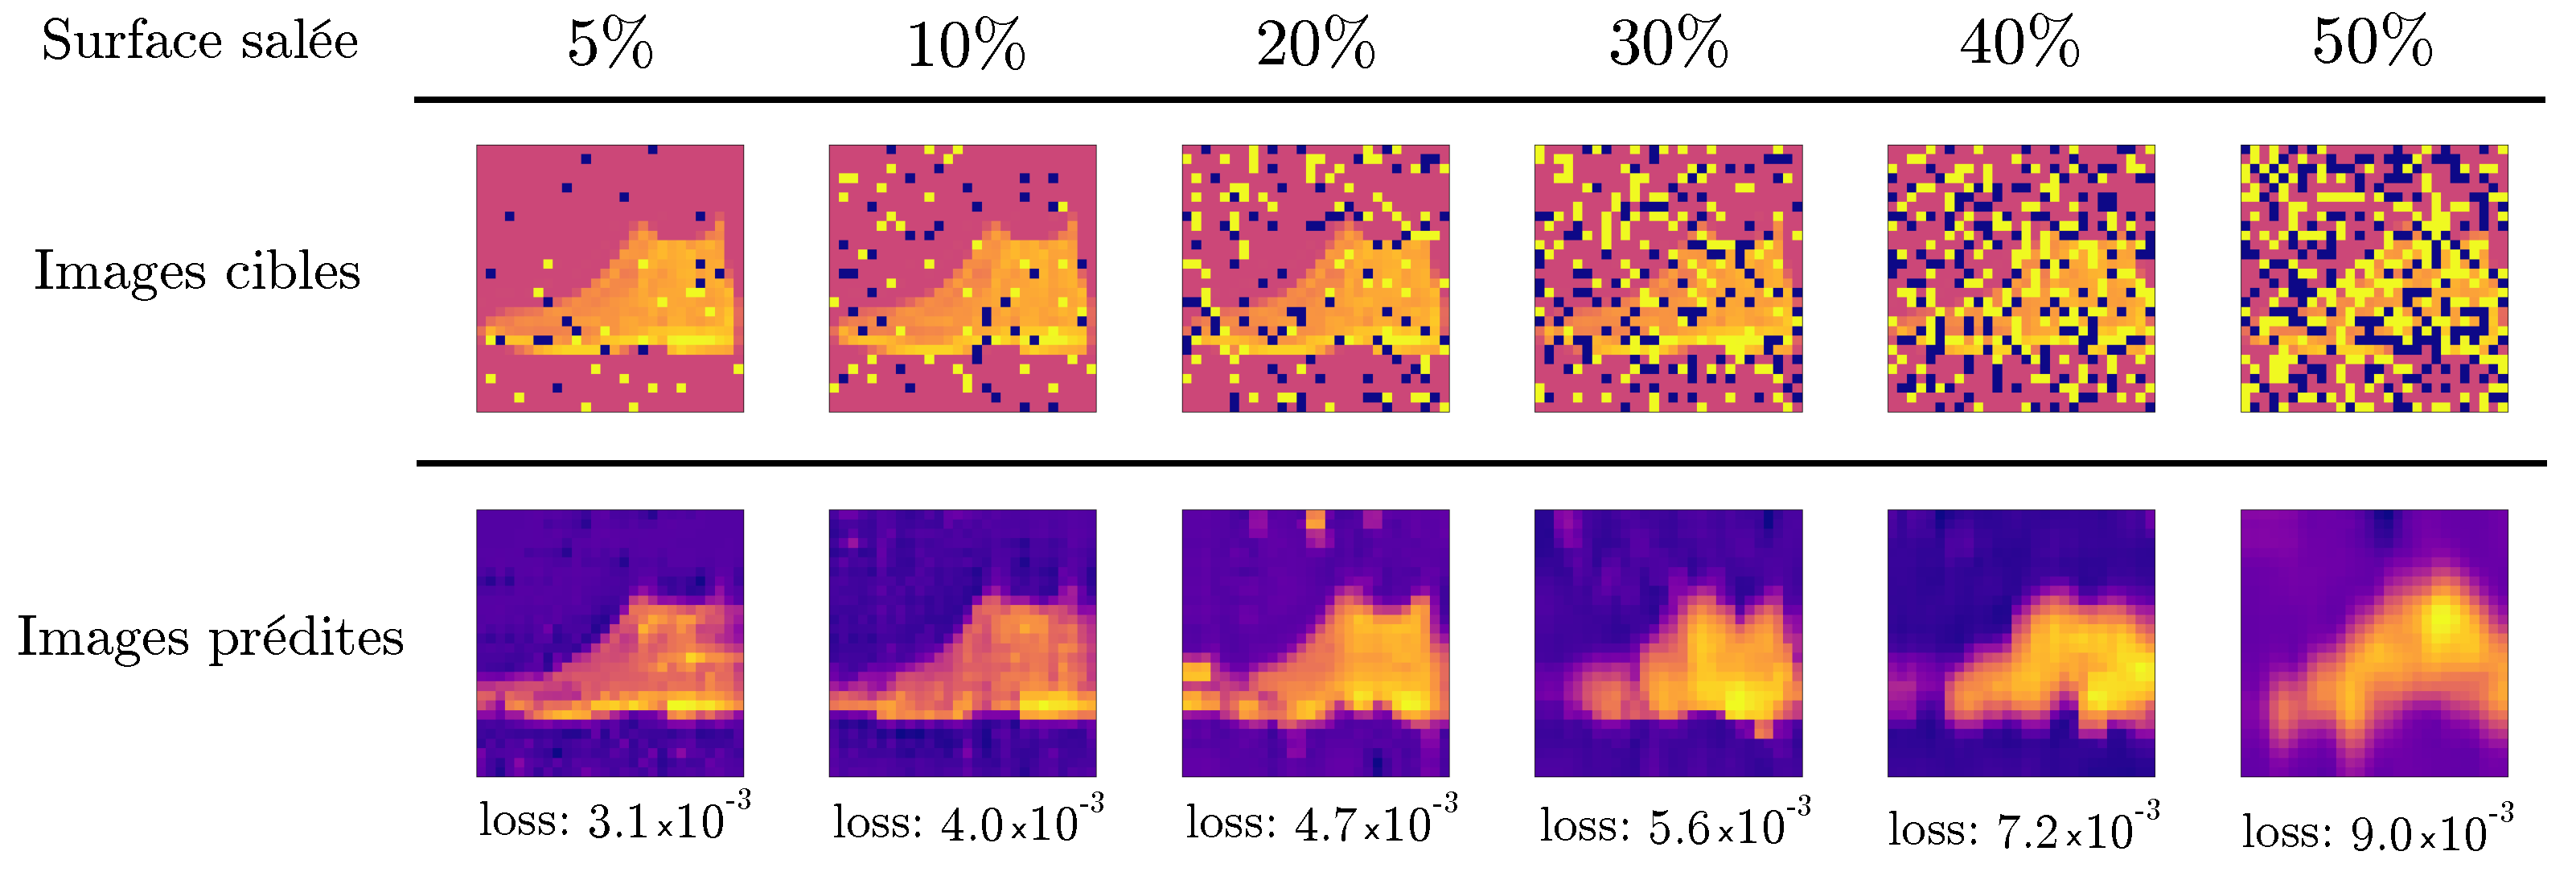
\includegraphics[width=0.90\linewidth]{parts/4-analyse_des_reseaux/others/figures/shoes_data.pdf}
    \vspace{1.2mm}
    \caption{ \centering Résultats de débruitage d'une image représentant une chaussure par le réseau $\mathcal{S}$MorphNetTanh à quatre couches entraîné sur FashionMNIST, avec plusieurs niveaux de bruit poivre et sel (en proportion de surface occupée).}
    \label{fig:debruitage}
  \end{center}
\end{figure}

\vspace{-0.8mm}
Malgré des valeurs de \textit{loss} plutôt élevées de l'ordre de $10^{-3}$ à $10^{-2}$, les résultats visuels de débruitage du réseau semblent plutôt bons à l'oeil nu : le réseau retrouve toujours globalement la forme de la chaussure, même à très haute proportion de bruit, et les pixels poivre et sel disparaissent très bien de l'image bruitée, même à 50\%. Une opération morphologique à la main ne pourrait faire que légèrement mieux. \\

\vspace{-1.0mm}
\noindent Cependant, bien que les résultats de débruitage semblent << plutôt bons >>, l'état du réseau l'est bien moins, car la forme des noyaux $w$ est très aléatoire et manque de régularité, et, surtout, les paramètres de contrôle $\alpha$ sont toujours très proches de 0. \\

%figure
%\vspace{-0.4mm}
\begin{figure}[htp]
  \begin{center}
    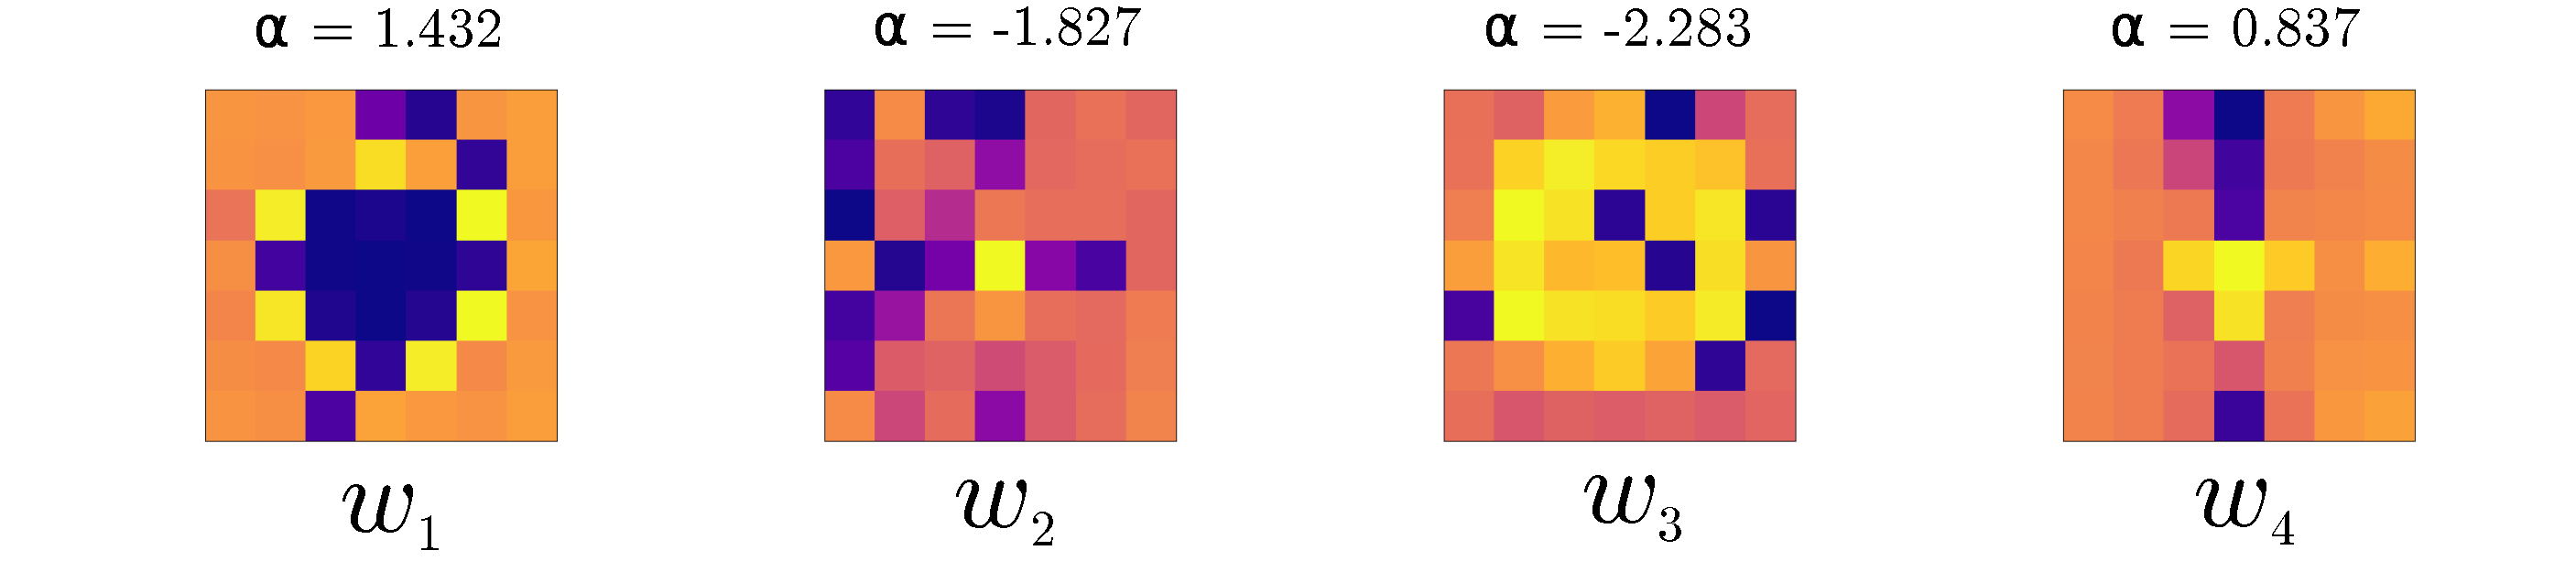
\includegraphics[width=0.80\linewidth]{parts/4-analyse_des_reseaux/others/figures/aaaaa.pdf}
    \vspace{-1.6mm}
    \caption{ \centering Noyaux $w$ et paramètres de contrôle $\alpha$ des quatre couches du réseau $\mathcal{S}$MorphNetTanh après entraînement sur FashionMNIST bruitée à 10\%.}
    \label{fig:aaaaa}
  \end{center}
\end{figure}

\vspace{-2.6mm}
La figure \ref{fig:aaaaa} ci-dessus présente l'état des quatre couches du réseau après un entraînement sur les images de la banque FashionMNIST bruitées à 10\%. D'après l'ordre des signes des $\alpha$, on peut en déduire que le réseau a le comportement d'une pseudo-fermeture suivie d'une pseudo-ouverture, ce que l'on visait initalement. Mais les $\alpha$ restent très proches de 0. On remarque sur les autres proportions de bruitage que plus cette proportion est élevée, plus les $\alpha$ sont proches de 0, et donc plus les couches ont le comportement d'un moyenneur, ce qui peut être observé sur la figure \ref{fig:debruitage}.
